%!TEX root = ../OpenNUI_Platform__Design_of_Smart_Space_Interaction_Platform.tex


\subsection{Experiments}

앞에서 제안한 특징점 Filtering 알고리즘을 이용하여 학습을 수행하였을 때 인식 성능의 개선을 측정하였다. 

실험 영상은, 서울시 가이드 지도 팜플릿 영상 16장을 선택하여 사용되었다. 이러한 영상을 rotation($0.5\sim2.0$배, 0.1배 간격), scale($0\degree\sim360\degree$, $10\degree$ 간격), blur(Gaussian blur, $r=0,3,5,7$pixels) 등의 변형(deformed)한 영상 32,256장 중 random sampling하여 train images 16,114장, test images 16,142장을 선택하였다.
먼저 train images에서 특징점들을 검출(detect)하고, detected keypoint 들을 이용하여 앞의 정의된 Score function($gf(p_i)$)을 계산하였다. 

특징점 데이터베이스는 Score function을 고려하지 않은 전체 특징점 집합($K_{all}, n(K_{all}) = 3000$)과, Score function에서 상위 50개, 100개, 300개, 500개 특징점들만 filtering 하여 구성한 특징점 집합($K_{50}, K_{100}, K_{300}, K_{500}$)으로 구성되었다. 

먼저 인식 속도 향상 정도를 측정하였다. 제안하는 방법은 train 단계에서 특징점들을 줄여 저장하기 때문에 비교 대상이 되는 특징점들의 개수가 줄어들게 된다. 이에 따라 연산의 속도가 향상되게 된다.

\todo{연산 속도 결과 삽입}
\label{fig:markerless_speed}
그림 \ref{fig:markerless_speed}에서 보듯이 연산 속도는 특징점 집합의 개수에 따라서 비례하여 향상되고 있다. 특히, 100개로 학습한 경우에서는 전체 특징점을 학습한 경우에 비하여 소요 시간이 $1/n$으로 감소됨을 볼 수 있다. Smart phone과 같이 경량화 된 실행 환경에서는 이렇게 연산량을 줄여줌으로써 빠른 interaction을 제공할 수 있게 된다.

제안하는 방법은 속도를 향상시키면서도 전체적인 인식성능의 향상도 기대할 수 있다. 이러한 특징점 데이터베이스를 이용하여 test images와의 인식 성능을 측정하였다. 인식 성능 측정을 위한 Match 방법은 \cite{choi_smart_2014}의 방법을 사용하여 false match를 최대한 억제하는 match 방법을 적용하였다.

이를 이용하여 인식율을 측정한 결과는 그림 \ref{fig:markerless_roc}와 같다. 전체 특징점 집합($K_{all}$)을 사용한 특징점 데이터베이스와 비교하여, $K_{500}$과 $K_{300}$은 조금 인식율의 저하가 보여졌으나, $K_{100}$과 $K_{50}$은 성능이 향상되었다. 
%%%%%분석 결과가 더 들어가면 좋겠다%%%%%

\begin{figure}[t!]
\centering
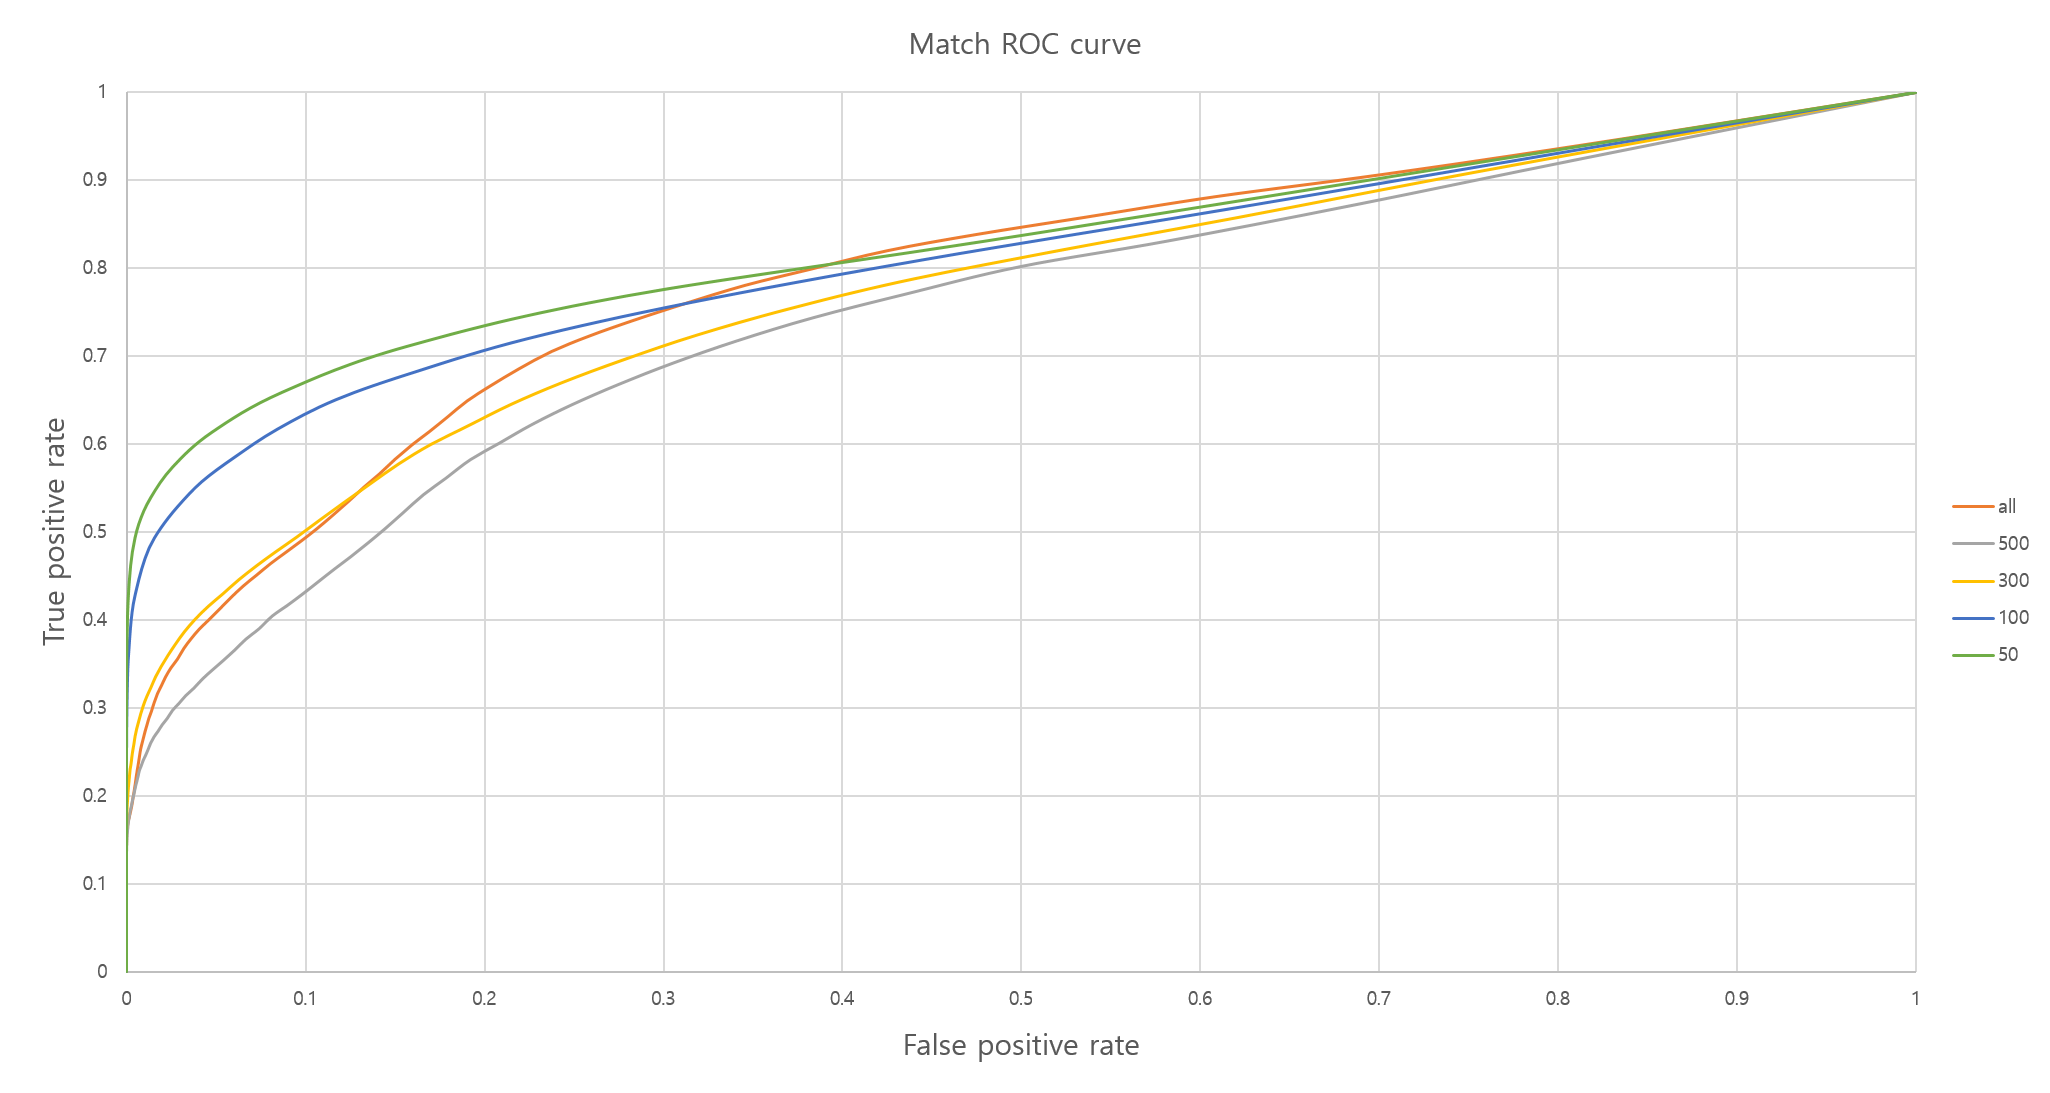
\includegraphics[width=1.0\textwidth]{4_MarkerlessAR/roc}
\caption{ROC curve for match rate}
\label{fig:markerless_roc}
\end{figure}

이러한 keypoint filtering을 수행하게 되면, miss-match를 유발하는 bad keypoint가 제거되기 때문에 match 결과의 reliability 가 높아진다. 이를 증명하기 위하여 Feature-level에서 Precision\cite{heinly_comparative_2012}을 계산하였다. Precision은 match 결과 구해진 correspondence pair의 수 대비 correct match의 비율로 계산이 된다. 이는 match 결과에 얼마나 miss-match가 적고 correct match의 비율이 높은지를 나타낸다. match 결과 대비 correct match의 비율이 높을수록 이후에 robust pose estimation의 성능에 영향을 미친다.

\begin{figure}[ht!]
\centering
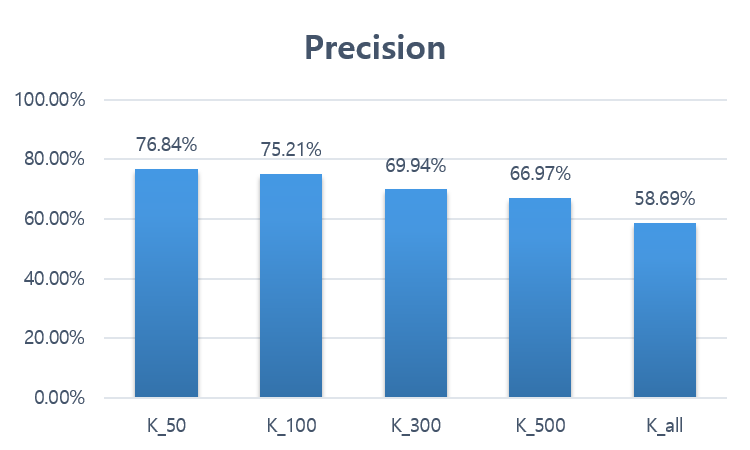
\includegraphics[width=1.0\textwidth]{4_MarkerlessAR/precision}
\caption{Precision of filtered keypoint database}
\label{fig:markerless_precision}
\end{figure}

\begin{table}[b!]
\centering
%\resizebox{\textwidth}{!}{%
\begin{tabular}{llllll}
\hline
\textbf{}                   & \textbf{$K_{50}$} & \textbf{$K_{100}$} & \textbf{$K_{300}$} & \textbf{$K_{500}$} & \textbf{$K_{all}$} \\
\textbf{Avg. Match Result}  & 10.098            & 15.618             & 26.747             & 31.409             & 44.859             \\
\textbf{Avg. Correct Match} & 7.759             & 11.747             & 18.705             & 21.033             & 26.326             \\
\textbf{Precision}          & 76.8\%            & 75.2\%             & 69.9\%             & 67.0\%             & 58.7\%             \\ \hline
\end{tabular}
%}
  \caption{Precision of filtered matching}
  \label{tab:markerless_precision}
\end{table}

Precision의 결과는 그림 \ref{fig:markerless_precision}와 표\ref{tab:markerless_precision}에 나타난다. 전체 특징점 집합($K_{all}$)에 비하여 filtered 특징점 집합들이 더 높은 precision을 나타내주었다. 검출되는 특징점의 개수는 줄어들지만, Correct Match의 비율이 높아지기 때문에 높은 Precision을 보여주었다. 이러한 결과는 robst pose estimation의 속도와 성능을 향상시킬 수 있다.

